%!LW recipe=pdflatex ➞ bibtex ➞ pdflatex`×2

\documentclass[twocolumn]{article} 

\title{TODO}
\author{Henry Ash Williams}
\date{\today}

\usepackage[backend=bibtex]{biblatex}
\usepackage[compact]{titlesec}
\usepackage{kpfonts}
\usepackage[margin=2cm]{geometry}
\usepackage{hyperref}
\usepackage{siunitx}
\usepackage{graphicx}
\usepackage[super]{nth}
\usepackage{tabularx}
\usepackage{ltablex}
\usepackage{subcaption}
\usepackage{longtable}
\usepackage{booktabs}
\usepackage{censor}
\usepackage{multirow}

\addbibresource{references.bib}

\begin{document}

\maketitle

\tableofcontents

\section{Introduction}

Propaganda is a covert technique in which one group attempts to manipulate the opinions, beliefs and attitudes of another without them realising it. This technique has been utilized extensively throughout history and is even seen in contemporary media. For example, shortly before the death of Augustus, the first emperor of Rome, an inscription was made on what was to be his final resting place. The inscription is known as ``The Deeds of the Divine Augustus'', and outlines both his religious power by describing himself as `Divine', and his importance to the Pax Romana, or the Roman Peace, by outlining his strategic ability through the anecdotes of his conquests found within the inscription. This was an attempt to shape the attitudes of his citizens towards him to be more favorable. In the years following his death, he was remembered as ``The Divine Augustus'', and was widely perceived with respect and reverence. However, during his reign, he routinely suppressed dissidents of the Roman Empire in an attempt to centralize his power. While it cannot be told whether the favorable view of Augustus within the Roman Empire was solely due to this text, this was not the only piece of propaganda he produced, and it likely helped to shape the view of his citizens, without them even noticing that their opinion was manufactured. 

This technique is not restricted to ancient history and is often seen in our modern media, whether we notice it or not. For example, in the lead-up to and during America's invasion of Iraq, US media reported on an alliance between Saddam Hussein and al-Qaeda to justify a US-led invasion of Iraq. The two groups were, however, largely at odds with each other, and no such allegiance was ever proven. Despite this, in 2002 a majority of Americans believed that Saddam Hussein was directly involved with both al-Qaeda and the 9/11 terror attacks. 

A majority of people who are exposed to propaganda do not recognize it as such, and considering the impacts of believing propaganda, both from a security and societal perspective can lead to significant consequences. However, by nature, propaganda is extremely difficult to detect, and many people struggle to recognize it even today. Considering the amount of media produced and consumed each day, a human approach to propaganda detection and classification is impossible, and new approaches are required. 

This paper will explore the effectiveness of modern machine learning models in both these tasks, namely the detection of propaganda within text, and the classification. Classification in this case refers to the methods of propaganda used within the text. This includes appealing to an individual's sense of fear, exaggerating facts, or the oversimplification of a complex topic. In this paper, we will cover my approaches to these tasks, using natural language processing techniques such as Term Frequency-Inverse Document Frequency, and Unigram Precision, as well as more complex, large language model approaches such as the fine-tuning of BERT models. 

\subsection{Propaganda Background}

According to~\textcite{scott1994power}, \emph{``Propaganda is a major form of manipulation by symbols''}. It can be found in reports by news or governments, films, social media, radio television, just to name a few. To better understand the scope of this problem, an in-depth understanding of how propaganda is used to manipulate within the context of this task. 

We were provided with a dataset of text samples and labels. The labels are a subset of the ones found in the dataset provided for Task 11 of the Semantic Evaluation 2020 workshop and include the appeal to fear prejudice, casual oversimplification, doubt, exaggeration and minimization, flag waving, loaded language, name calling and labeling, and repetition. 

The appeal to fear prejudice seeks to manipulate the opinions of the target audience by provoking panic among them and is likely one of the most effective techniques to manufacture opinions~\cite{tannenbaum2015appeal}. This can be seen throughout history, one of the best examples of this is Joeseph Gobbel's usage of the technique to convince the German public that the Allies wanted to exterminate the German people during the reign of the Nazi party. 

Casual oversimplification assumes a single cause or reason for an issue despite the reality being far more complex~\cite{da-san-martino-etal-2020-semeval}. This could include blaming societal issues on a single group of people.  

Within propaganda, doubt is used to influence perception by encouraging its targets to question the legitimacy of others. This could take the form of an advertiser shaping the perception of a competing brand's effectiveness. Thus, encouraging the target to buy their product instead. 

Exaggeration and minimization unsurprisingly, is the opposite of casual oversimplification. This is often seen in advertising, where brands exaggerate claims about their products to make them seem better than those of their competitors. Minimization is very similar to this, whereby a brand may make problems with their products seem like less of an issue than they are. They are grouped in the dataset due to their relatively low frequency, and the commonalities between them. 

Flag waving utilizes strong nationalistic views to promote actions or ideas~\cite{hobbs2014teaching}. To re-use the advertiser example, it could be promoting the idea that their brand's product is better because it is manufactured in a certain country.

Name-calling and labeling are grouped as well, as they are very similar. These techniques assign the object of the propaganda campaign (the entities which the propaganda campaign seeks to manipulate individuals' perceptions) a name that the targets would find undesirable. This could be a brand calling a competitor's product an imitation, which most people would dislike. 

Repetition involves repeating a message over and over again until the targets accept it as true. 

\section{Methods}


\subsection{Data Analysis}

\begin{table*}[t!]
    \centering
    \begin{tabular}{@{}clccc@{}}
        \toprule
        \multicolumn{2}{c}{\textbf{Label}} & \multicolumn{3}{c}{\textbf{Metrics}} \\ \midrule
        \textbf{ID}& \textbf{Description} & \textbf{Mean} & \textbf{Std} & \textbf{Range} \\ \bottomrule
        \textbf{1} & Appeal To Fear Prejudice & 39.65 & 17.38 & 107 \\
        \textbf{2} & Name Calling, Labelling & 44.49 & 23.15 & 144 \\
        \textbf{3} & Exaggeration, Minimisation & 40.03 & 18.86 & 87 \\
        \textbf{4} & Not Propaganda & 30.02 & 15.25 & 131 \\
        \textbf{5} & Loaded Language & 37.72 & 18.49 & 93 \\
        \textbf{6} & Casual Oversimplification & 43.58 & 21.96 & 132 \\
        \textbf{7} & Doubt & 41.65 & 25.45 & 159 \\
        \textbf{8} & Repetition & 34.42 & 18.6 & 120 \\
        \textbf{9} & Flag Waving & 40.0 & 18.63 & 112 \\ 
        \bottomrule
    \end{tabular}
    \caption{Labels found within the dataset, and metrics relating to the word count of the text samples}
    \label{tab:dataset-metrics}
\end{table*}

To develop a model capable of achieving the goals outlined in the previous section, we need a thorough understanding of the data we've been provided with. The dataset of text samples, some of which contained propaganda, and others that didn't. Overall, there were 3,200 samples, 50\% of which contained propaganda, and 50\% of which didn't. It came in the form of two separate tab-separated value files, one for training, and another for testing. The testing dataset contains 640 samples, 48\% of which contain propaganda. The training dataset contains 2,560 samples, 52\% of which contained propaganda. 

There are 9 labels, including one for samples without propaganda. The average word count, as well as the standard deviation, and range of each class is displayed in~\autoref{tab:dataset-metrics}. As we see, the average length of each sample across the various propaganda classes is approximately 39 words. However, some classes such as name calling and labeling, and casual oversimplification on average exhibit longer sequences. Despite this, we see little correlation between word count within the samples and the label assigned to them. 

Within each of the text samples, there are tags indicating the area of interest. This indicates where the propaganda is within the sample. We extracted the text within this area of interest and calculated the same metrics as we did for~\autoref{tab:dataset-metrics}. The results of this are demonstrated in~\autoref{tab:extracted-metrics}. While they exhibit a correlation between the number of words in the sample, and a the correlation isn't very strong, and likely shouldn't be used to predict and classify propaganda.

\begin{table}[h]
    \centering
    \begin{tabular}{@{}cccc@{}}
        \toprule
        \multicolumn{1}{c}{\textbf{Label}} & \multicolumn{3}{c}{\textbf{Metrics}}          \\ \midrule
        \multicolumn{1}{c}{\textbf{ID}}    & \textbf{Mean} & \textbf{Std} & \textbf{Range} \\ \midrule
        \textbf{1} & 23.72 & 14.75 & 87 \\
        \textbf{2} & 22.95 & 19.99 & 159 \\
        \textbf{3} & 3.14 & 4.08 & 38 \\
        \textbf{4} & 19.24 & 13.61 & 79 \\
        \textbf{5} & 8.15 & 6.2 & 46 \\
        \textbf{6} & 7.26 & 8.01 & 92 \\
        \textbf{7} & 12.04 & 13.27 & 78 \\
        \textbf{8} & 4.8 & 3.92 & 23 \\
        \textbf{9} & 3.72 & 3.7 & 29 \\
        \bottomrule
        \end{tabular}
    \caption{Metrics of text samples with area of interest extraction}
    \label{tab:extracted-metrics}
\end{table}

In order to demonstrate the effectiveness of my approach, it is first necessary to establish a baseline for performance. In this case, the baseline would be randomly selecting a label for a given sample. For classification, the baseline is 50\% and for classification, as there are 8\footnote{The inputs to this model are known to contain propaganda, so we can disregard} labels to choose from, the baseline accuracy is around 12.5\%. 

\subsection{Detection}

Propaganda detection is a binary classification task, meaning the output of the system will be one of two values. In this case, 1 indicates the text sample contains propaganda, and 0 indicates the lack of propaganda within the sample. There are several approaches to text-based binary classification such as bag-of-word-based approaches, which make use of a vocabulary of all unique words in the training data, and then a machine learning algorithm such as Naive Bayes or Support Vector Machines to perform classification.

\subsubsection{Bag of Word classifier}

A bag of words approach first requires us to pre-process our training data. This typically involves tokenization, where text is split into individual words, converting the tokens to lowercase, removal of stopwords (words that do not carry significant meaning such as ``the'', ``and'', ``is'', etc), and the lemmatization of the remaining words. 

In Linguistics, a Lemma is the base form of a word. For example, the words ``running'', ``ran'', ``runs'' are all lexemes of the lemma ``run''. The process of converting a given lexeme to its base form, i.e. its' lemma, is known as lemmatization and is a critical step of data preprocessing within the development of bag-of-word classifiers. This is because it significantly reduces the dimensionality of the set of words, which thereby reduces the complexity of the classifier. For example, the training data has 3261 unique words that are classified as propaganda, upon performing lemmatization on these words, there are 3043 words. Furthermore, when it comes time to perform inference using our model, we don't want to miss a word within the known propaganda words dataset simply because it's in a different form. This requires us to perform the above pre-processing steps on our test data for our training data. 

To determine the class of a given sample, we can simply check how many words are common between our bag of words, and the sample we want to test, divided by the total number of words in the sample. This value is fed into a simple logistic regression algorithm, which then makes a prediction. The results for this approach are demonstrated in~\ref{tab:detection-results}. 

\begin{figure}[ht]
    \centering 
    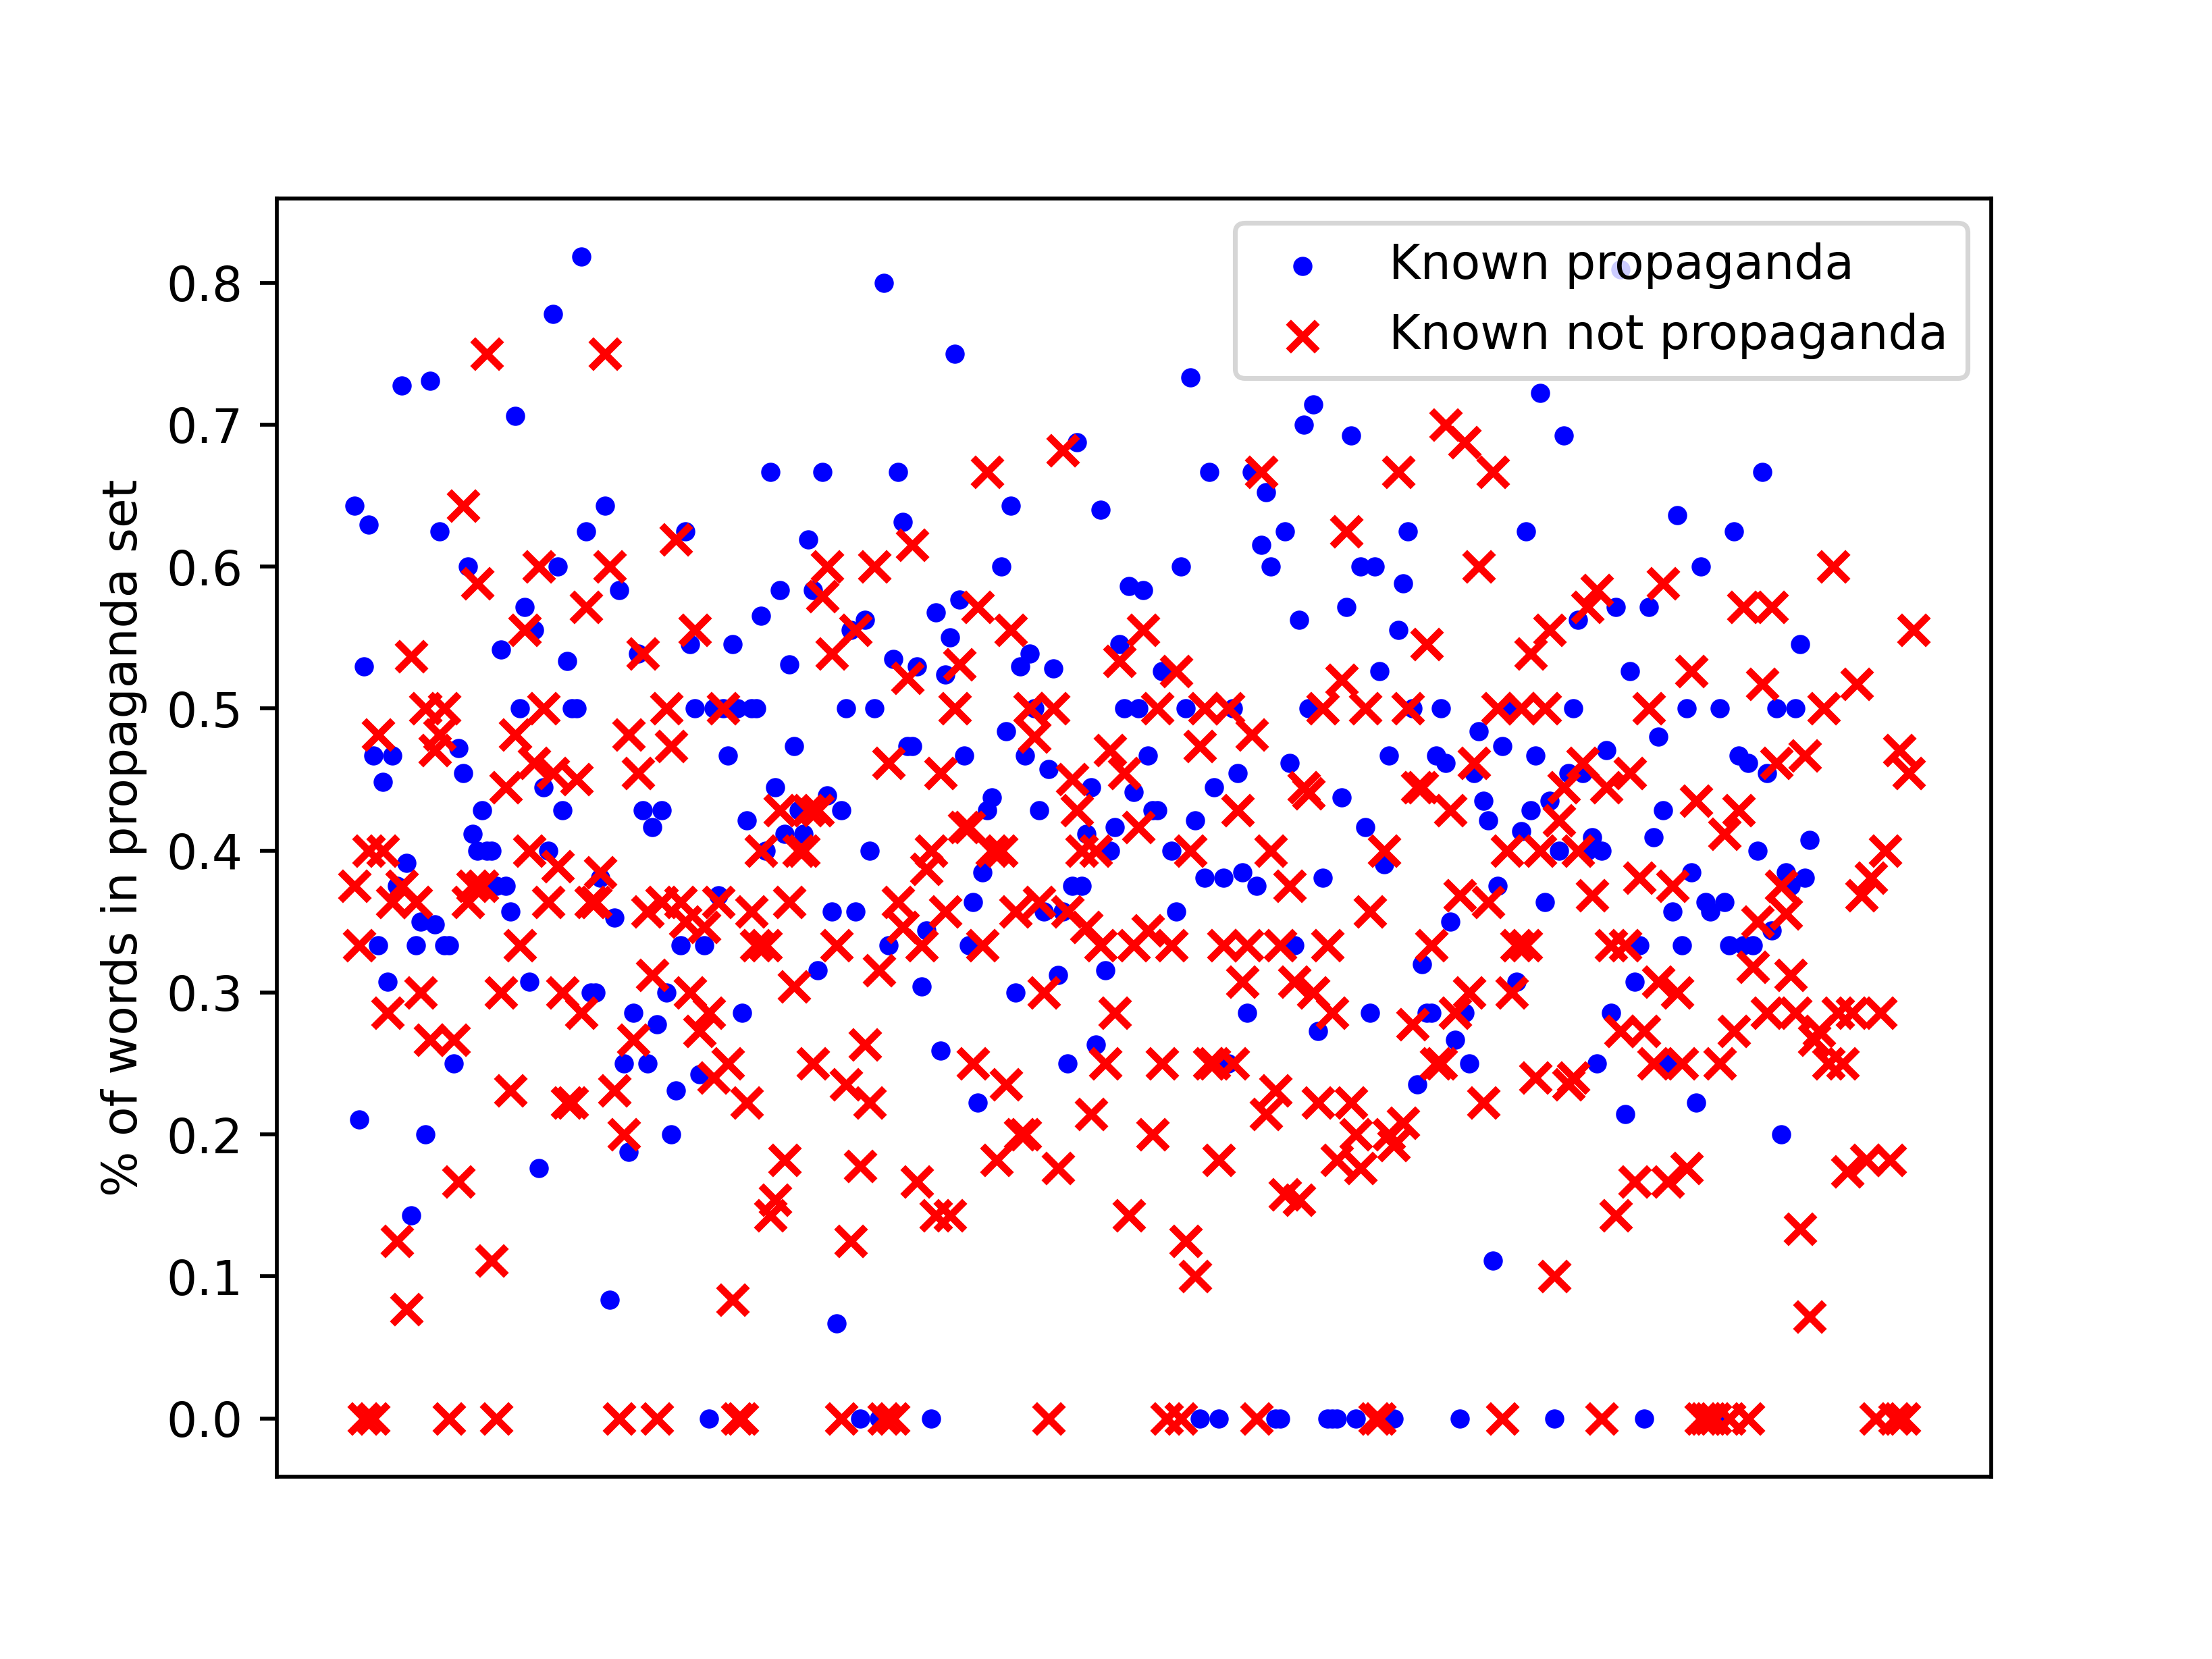
\includegraphics[scale=0.5]{../assets/bag-of-words-correlation.png}
    \caption{Correlation between percentage of words in common with propaganda set, and known classification}
    \label{fig:bag-correlation}
\end{figure}

I chose to experiment with this model, as it offers a solid baseline for further development. It also is very simple to get up and running quickly. However, its performance is slightly above our random baseline, achieving a 60\% test accuracy. To understand why the accuracy was so low, I analysed the correlation between the number of words shared between test samples, and the set of words commonly found in propaganda. This analysis is shown in~\autoref{fig:bag-correlation}, and we see that there is very little correlation between the overlap of words found in the test sample and the words in the propaganda set, and the label assigned to the test sample explaining the low accuracy of the model. 

\subsubsection{Term Frequency-Inverse Document Frequency and Support Vector Machines}

I then went on to enhance this model using Term Frequency-Inverse Document Frequency, TF-IDF. This approach adds additional information in the form of the word importance within the corpus based on how often it occurs. By transforming the training dataset. The relative frequency of a given term $t$ within a document $d$ of a corpus $D$ is calculated using the expression found in~\autoref{eq:tfidf}, where $f_{t, d}$ is the number of occurrences of the term $t$ in the document $d$, and $\sum_{t'\in d} f_{t', d}$ is the total number of terms in $d$.

\begin{figure}
    \begin{align*}
        \text{TF}(t, d) &= \frac{f_{t, d}}{\sum_{t' \in d}f_{t',d}} \\ 
        \text{IDF}(t, D) &= \log \left( \frac{|D|}{1 + |\{d \in D : t \in d\}|} \right) \\ 
        \text{TF-IDF}(t, d, D) &= \text{TF}(t, d) \cdot \text{IDF}(t, D) 
    \end{align*}
    \caption{How a term's relative frequency within a document given a corpus is calculated using TF-IDF.}
    \label{eq:tfidf}
\end{figure}

The training dataset is then to its TF-IDF representation, which a support vector machine was then trained on. A support vector machine is similar to the logistic regressor used in the bag of words approach as it finds a hyperplane that separates the two classes. However, it seeks to maximize the distance of the margin between them. The margin is the distance between the hyperplane and its closest data point on either side of its decision boundary. This allows support vector machines to better generalize the task and prevents overfitting. A kernel is used to transform the input space in cases where the data is not linearly separable. To determine the best configuration of this approach, I evaluated the model's accuracy on each of them. I found that on average, sigmoid, linear, and radial basis function (RBF) kernels are optimal for this task, reaching 73\% test accuracy. These results were obtained over 10 iterations to reduce the presence of outliers within the data. The results I gathered for this are demonstrated in~\autoref{tab:results}.

\subsubsection{Bidirectional Encoder Representation from Transformers}

I then went on to test the effectiveness of the Bidirectional Encoder Representation from Transformers (BERT) large language model introduced by researchers at Google. This model uses an ``encoder only'' transformer architecture. Encoders are responsible for learning and extracting relevant information from the input text, and outputs an embedding. These embeddings include a one-hot vector of the input token, a positional encoding, and a token type. It has a contextual understanding of text, can consider words on either side of the current word, and demonstrates excellent performance on similar tasks. 

When applying BERT to a new problem, an approach known as transfer learning is used. This is where a trained model is re-trained on a new task. This allows us to significantly decrease the time spent training, and the amount of data necessary for it. When applying the pre-trained model to this task, it demonstrates the worst performance out of all the models I've tested, even falling behind our baseline of randomly picking labels. However, after performing training for 10 epochs, taking approximately 10 minutes on an Apple Macbook Pro with an M2 Pro chip, and 16GB of memory, it quickly surpasses the bag of words classifier in terms of performance, see~\autoref{tab:results}. To further enhance the performance of this model, I performed a technique known as Bayesian hyperparameter optimization. Hyperparameters are first selected randomly, then find either the parameters with the best performance or the point that has the highest potential to achieve a better result, the point with the highest uncertainty. 

I first trained my model using the following hyperparameters: a batch size of 32, a learning rate of 2e-5, a weight decay of 0.01, a dropout rate of 0.1 and the Adam optimization function. After training for 5 epochs, this model achieved approximately 70\% test accuracy. However, after hyperparameter optimization, I was able to achieve 80\% test accuracy. These results are shown in the~\autoref{fig:detection-cm}. The most significant parameter to the performance of the model was the optimzation function used by the model. For example, no models trained using the RMSprop optimizer achieved better than a 0.44 test f1 score, and models trained using the Adam optimizer did not achieve better than a 0.41 test f1 score. However, models trained using stochastic gradient descent were able to reach up to a 0.80 test f1 score. Weight decay and dropout rate does not seem to have much of an impact on performance, as the best-performing models all had a wide variety of values, for example the dropout values ranged from 0.1174 and 0.3859, and weight decay ranged from 0.002 to 0.009. Learning rate, however, had a much smaller range for these top-performing models, from 0.04 to 0. Most of the values within this range are clustered towards 0.01 leading me to believe it should be extremely small.

\begin{figure}
    \centering 
    \includegraphics*[scale=0.25]{../assets/propaganda-detection-confusion-matrix.png}
    \caption{The confusion matrix of the propaganda detector}
    \label{fig:detection-cm}
\end{figure}

\subsection{Classification}

Classification is a more challenging task. We are given the region of interest from within a text sample. This sample is known to contain propaganda. Therefore, we only have 8 labels to consider. I begun by applying the same TFIDF technique to the problem. This resulted in an accuracy and f1 score of 50\%. Considering the baseline for this task would be an accuracy of approximately 12\% and an F1 score of approximately 0.14, the TFIDF+SVC model provides decent performance. However, there is still room for improvement. 

I chose to re-use the BERT model for the classification task, as it demonstrated excellent performance in the first task, after hyperparameter optimization. I took the same approach to pre-processing the training data as I did for the pre-processing task, using the BERT tokenizer. However, I did remove all samples without propaganda present, as they are not considered in this task. I also chose to use the same hyperparameters to begin with. This model achieved 46\% accuracy. As demonstrated in the previous task however, there is room to improve this metric. 

To improve the performance of this model, I again performed a hyperparameter sweep. I ran this sweep on an RTX 4090\footnote{Special thanks to my housemate Byron who let me use his PC for this}, which allowed me to train the model over 100 times in under 2 hours. The best performing model I trained during this sweep, achieved a test accuracy of 69\%, using the stochastic gradient descent optimzer, a batch size of 64, a dropout rate of 0.21, a learning rate of 0.02, and a weight decay value of 0.009. The confusion matrix for this model is displayed in~\ref{fig:classification-cm}. 

\begin{figure}
    \centering
    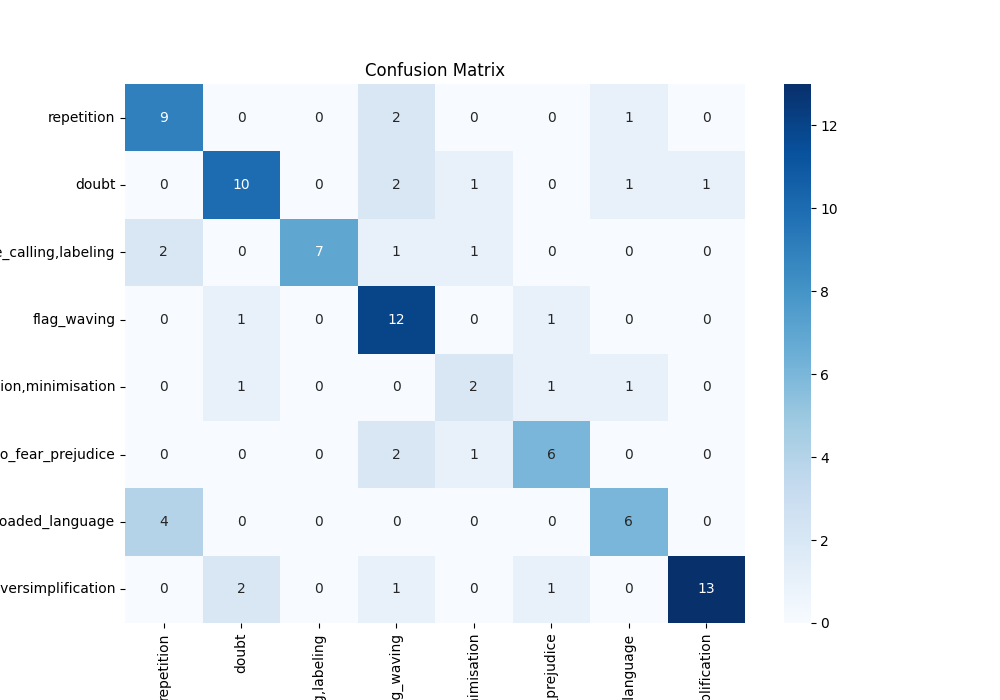
\includegraphics[scale=0.3]{../assets/propaganda-classification-confusion-matrix.png}
    \caption{The confusion matrix of the propaganda classification model.}
    \label{fig:classification-cm}
\end{figure}

\section{Evaluation}

\begingroup
\setlength{\tabcolsep}{10pt} % Default value: 6pt
% \renewcommand{\arraystretch}{1.25} % Default value: 1

\begin{table*}[t]
    \centering
    \begin{tabular}{@{}cccccc@{}}
        \toprule
        \textbf{Task} & \textbf{Method} & \multicolumn{4}{c}{\textbf{Performance}} \\ \midrule
        & & Accuracy & F1 Score & \multicolumn{1}{l}{Precision} &\multicolumn{1}{l}{Recall} \\ \midrule

        1 & Random Baseline & 0.48 & 0.49 & 0.49 & 0.49 \\
        1 & \begin{tabular}[c]{@{}c@{}}
            Bag-of-Words \\ Logistic Regression
        \end{tabular} & 0.61 & 0.64 & 0.61 & 0.61 \\
        1 & \begin{tabular}[c]{@{}c@{}}
            TF-IDF SVC \\ 
            (With linear kernel)
        \end{tabular} & 0.72 & 0.72 & 0.72 & 0.72 \\
        1 & \begin{tabular}[c]{@{}c@{}}
            TF-IDF SVC \\ 
            (With polynomial kernel)
        \end{tabular} & 0.66 & 0.65 & 0.64 & 0.65 \\
        1 & \begin{tabular}[c]{@{}c@{}}
            TF-IDF SVC \\ 
            (With rbf kernel)
        \end{tabular} & 0.73 & 0.73 & 0.73 & 0.73 \\
        1 & \begin{tabular}[c]{@{}c@{}}
            TF-IDF SVC \\ 
            (With sigmoid kernel)
        \end{tabular} & 0.72 & 0.72 & 0.72 & 0.72 \\
        1 & BERT Baseline & 0.51 & 0.34 & 0.26 & 0.51 \\
        1 & Fine-Tuned BERT & 0.63 & 0.63 & 0.63 & 0.63 \\
        1 & \begin{tabular}[c]{@{}c@{}}
            Fine-Tuned BERT\\ 
            With Hyperparameter Optimization
        \end{tabular} & 0.8 & 0.8 & 0.81 & 0.8 \\ 
        2 & Random Baseline & 0.12 & 0.14 & 0.3 & 0.12 \\
        2 & \begin{tabular}[c]{@{}c@{}}TF-IDF SVC \\ (With sigmoid kernel)\end{tabular} & 0.5 & 0.5 & 0.53 & 0.5 \\
        2 & BERT Baseline & 0.11 & 0.04 & 0.03 & 0.1 \\
        2 & Fine-Tuned BERT & 0.46 & 0.43 & 0.47 & 0.46 \\
        2 & \begin{tabular}[c]{@{}c@{}}Fine-Tuned BERT\\ With Hyperparameter Optimization\end{tabular} & 0.69 & 0.7 & 0.72 & 0.69 \\ \bottomrule
    \end{tabular}
    \caption{The results and key metrics of my approaches for the both tasks, task 1 being detection of propaganda, task 2 being its classification}
    \label{tab:results}
\end{table*}
\endgroup

\section{Conclusion \& Further Work}

\printbibliography
\end{document}